\textcolor{cyan}{\chapter{Les bases mathématiques pour le Machine Learning}}
%{État des connaissances}
\section{Eléments de calcul différentiel}
	Cette section est inspirée des notes écrites par le Professeur TSHIMANGA \cite[voir][page:45-82]{jtshiman:2021} et de consignes données
	par .... [ voir ?, page:..-..].
	\subsection{Convexité}
	\paragraph*{Définition : (Ensemble convexe)}
	Une partie $\mathcal{C} \subset \mathbb{R}^n $ est dite convexe si et seulement si pour tout $(x,y) \in \mathcal{C}^2$,
	et pour tout $ \alpha \in [0, 1]$,
	$$ \alpha x + (1 - \alpha)y \in \mathcal{C}$$ combinaison convexe.
	\begin{figure}
	\centering
	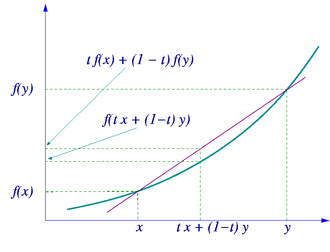
\includegraphics{images/convex_function_graph.png}
	\caption{Fonction convexe (image de Wikipédia)}
	\label{convexe_graph}
	\end{figure}
	\paragraph*{Définition : (Fonction convexe)}
	Une fonction $f$ d'un intervalle réel $I \in \mathcal{C}$ est dite fonction convexe lorsque, $\forall (x,y)$ de $I$ tel que $(x,y) \in \mathcal{C}^2$ et tout $\alpha \in [0, 1]$ on a :
	
	%Une fonction $f$ définie sur une partie $\mathcal{C}$ convexe est une fonction convexe dans $\mathcal{C}$ ssi $(x,y) \in \mathcal{C}^2$, et pour tout $\alpha \in [0, 1]$ on a,
	
	\begin{equation}
	f(\alpha x + (1 - \alpha)y) \leq \alpha f(x) + (1 - \alpha)f(y)
	\label{eq_convexe-1}
	\end{equation}
	et si
	\begin{equation}
	f(\alpha x + (1 - \alpha)y) < \alpha f(x) + (1 - \alpha)f(y)
	\label{eq_convexe-2}
	\end{equation}
	on dit que la fonction est strictement convexe dans $\mathcal{C}$\\\\
	Ex:
	\begin{itemize}
	\item[--] La fonction $ f(x) = x^2$ est convexe.
	\item[--] La fonction $ f(x) = x^T x$ est convexe.
	\item[--] La fonction $ f(x) = x^T Ax$ est convexe, ssi A est symétrique semi-définie positive.
	\end{itemize}
	
	
	\subsection{Développement limité}\label{dev_lim}
	Lorem ipsum dolor sit amet, consectetur adipiscing elit, sed do eiusmod tempor incididunt ut labore et dolore magna aliqua.
	\subsubsection{Différentiabilité au sens de Frechet}
	??? paler de son implication dans le gradient
	Lorem ipsum dolor sit amet, consectetur adipiscing elit, sed do eiusmod tempor incididunt ut labore et dolore magna aliqua. Ut enim ad minim veniam, quis nostrud exercitation ullamco laboris nisi ut aliquip ex ea commodo consequat. Duis aute irure dolor in reprehenderit in voluptate velit esse cillum dolore eu fugiat nulla pariatur. Excepteur sint occaecat cupidatat non proident, sunt in culpa qui officia deserunt mollit anim id est laborum.
	
	\subsection{Fonctions dérivables}
	
	\subsubsection{Gradient}\label{grad}
	\paragraph*{Définition:}Le gradient d'une fonction de plusieurs variables en un certain point est un vecteur qui caractérise la variabilité de cette fonction au voisinage de ce point. Défini en tout point où la fonction est différentiable, il définit un champ de vecteurs, également dénommé gradient. Le gradient est la généralisation à plusieurs variables de la dérivée d'une fonction d'une seule variable.\\ \\
	\paragraph*{Définition mathématique :} Dans un système de coordonnées cartésiennes, le gradient d'une fonction {$ f(x_{1},x_{2},\dots ,x_{n}$)} est le vecteur de composantes {$ \partial f/ \partial x_{i}\ (i=1,2,\dots ,n)$}, c'est-à-dire les dérivées partielles de $f$ par rapport aux coordonnées.
	$${\nabla f(x)={
	\begin{bmatrix}
	{\frac {\partial f(x)}{\partial x_{1}}}\\
	\vdots \\
	{\frac {\partial f(x)}{\partial x_{n}}}
	\end{bmatrix}}} \in \mathbb{R}^n $$
	\paragraph*{Gradient sous forme de développement limité:}
	\textit{Si une application admet un gradient en un point, alors on peut écrire ce développement limité du premier ordre (voir le point \ref{dev_lim})}
	
	$${
	f(x+h)=f(x)+\langle \nabla f(x)\mid h\rangle +o(h)
	}$$
	ou
	$$ {
	f(x-h)=f(x)-\langle \nabla f(x)\mid h\rangle +o(h)
	}$$
	\textit{Numériquement, il est très intéressant de faire ensuite la demi-différence des deux développements pour obtenir la valeur du gradient et on note que celui-ci ne dépend pas en fait de la valeur de la fonction au point $x : f (x)$. Cette formule a l'avantage de tenir compte des gradients du 2e ordre et est donc beaucoup plus précise et numériquement robuste. L'hypothèse est, en pratique, de connaitre les valeurs "passé" et "futur" de la fonction autour d'un petit voisinage du point $x$}.\\
	\paragraph*{Définition numérique:}
	Une fonction multivariée (a variable vectorielle)
	$ f(x)	: \mathbb{R}^n \rightarrow \mathbb{R} : x \rightarrow f(x) $ définie sur un ouvert $O \in \mathbb{R}^n$ est dite dérivable (au sens de Fréchet??) en $x$ ssi il existe un vecteur noté $\nabla f(x) \in \mathbb{R}^n$ tel que
	\begin{equation}
	f(x+h) = f(x) + \nabla f(x)^{T}h + o(||h||)
	\end{equation}
	
	$\nabla f(x) \in \mathbb{R}^n$ et où l’on a posé que le reste $o(||h||) = ||h||\epsilon (h) \in \mathbb{R}^n$, avec $h \in \mathbb{R}^n$
	\begin{center}
	$\epsilon (h): \mathbb{R}^n\rightarrow \mathbb{R}, \hspace{1 cm} \lim\limits_{||h|| \rightarrow 0} \epsilon(h)=0$.
	\end{center}
	Le vecteur $\nabla f(x)$ est unique et s’appelle \textbf{gradient} de $f(x)$ en $x$.
	Le gradient s’adresse aux fonctions scalaires à variables vectorielles.
	\paragraph*{A propos de la notation $\textbf{o(||h||)}$:}
	La notation de Landau $o(||h||)$ traduit le comportement d’une fonction de $h$ qui [est ??] tend vers $0$ d’un ordre de grandeur plus vite que $||h||$.\\\\
	Elle est infiniment plus petit que $h$ dans le voisinage de $0$
	
	
	
	
	\subsubsection{Hessienne}
	\paragraph*{Définition mathématique:}
	Etant donnée une fonction ${f}$ à valeurs réelles
	
	$${ f:\mathbb{R}^{n}\to \mathbb {R} ;(x_{1},...,x_{n})\mapsto f(x_{1},...,x_{n})}$$
	dont toutes les dérivées partielles secondes existent, le coefficient d'indice ${ i,j}$ de la \textbf{matrice hessienne\footnote{En mathématiques, la matrice hessienne (ou simplement la hessienne) d'une fonction numérique $f$ est la matrice carrée, notée $H(f)$, de ses dérivées partielles secondes.}} ${H(f)}$ vaut ${H_{ij}(f)={\frac {\partial ^{2}f}{\partial x_{i}\partial x_{j}}}}$.\\
	Autrement dit,
	$$
	{ H(f)={
	\begin{bmatrix}{
	\frac {\partial ^{2}f}{{\partial x_{1}}^{2}}}&{\frac {\partial ^{2}f}{\partial x_{1}\partial x_{2}}}&\cdots &{\frac {\partial ^{2}f}{\partial x_{1}\partial x_{n}}}\\
	{\frac {\partial ^{2}f}{\partial x_{2}\partial x_{1}}}&{\frac {\partial ^{2}f}{{\partial x_{2}}^{2}}}&\cdots &{\frac {\partial ^{2}f}{\partial x_{2}\partial x_{n}}}\\
	\vdots &\vdots &\ddots &\vdots \\
	{\frac {\partial ^{2}f}{\partial x_{n}\partial x_{1}}}&{\frac {\partial ^{2}f}{\partial x_{n}\partial x_{2}}}&\cdots &{\frac {\partial ^{2}f}{{\partial x_{n}}^{2}}}
	\end{bmatrix}}} .
	$$
	
	\paragraph*{Définition numérique:}
	Supposons que $f : \mathbb{R}^{n} \to \mathbb{R}$ définie sur un ouvert $\mathcal{O} \in \mathbb{R}^{n}$. La fonction $f(x)$ est dite 2
	fois continûment dérivable (au sens de Fréchet??) si en tout $x \in \mathcal{O}$ on a
	
	\begin{equation}
	f(x + h) = f(x)+\nabla f(x)^Th + \frac{1}{2}h^T\nabla^2f(x)h+o(||h||^2)
	\end{equation}
	avec$\nabla f(x)\in \mathbb{R}^{n\times n}$ et où on a posé que le reste
	$ o(||h||^2) =||h|| \epsilon(h) \in \mathbb{R} $ avec
	$\lim\limits_{||h|| \to 0} \epsilon(h) = 0 $
	La matrice carrée symétrique $\nabla^2 f(x)$ appelée \textbf{Hessien} de $f(x)$ en $x$. Remarque :
	
	$$
	\lim\limits_{||h|| \to h} \frac{o(||h||^2)}{||h||} = 0  \in \mathbb{R}
	$$
	La Hessienne s’adresse aux fonctions scalaires à variables vectorielles.
	
	\subsubsection{Jacobienne}
	\paragraph*{Définition mathématique:}
	Soit F une fonction d'un ouvert de $\mathbb{R}^{n}$ à valeurs dans $\mathbb{R}^{m}$ ($F:\mathbb{R}^{n}\to \mathbb {R}^{m}$). Une telle fonction est définie par ses $m$ fonctions composantes à valeurs réelles :
	
	$$
	{ F:
	{\begin{pmatrix}
	x_{1}\\\vdots \\
	x_{n}
	\end{pmatrix}}
	\longmapsto
	{\begin{pmatrix}
	f_{1}(x_{1},\dots ,x_{n})\\
	\vdots \\f_{m}(x_{1},\dots ,x_{n})
	\end{pmatrix}}}.
	$$
	Les dérivées partielles de ces fonctions en un point $M$, si elles existent, peuvent être rangées dans une matrice à $m$ lignes et $n$ colonnes, appelée \textbf{matrice jacobienne\footnote{En analyse vectorielle, la matrice jacobienne est la matrice des dérivées partielles du premier ordre d'une fonction vectorielle en un point donné.}} de $F$ :
	$$
	J_{F}\left(M\right)={
	\begin{pmatrix}
	{\dfrac {\partial f_{1}}{\partial x_{1}}}&\cdots &{\dfrac {\partial f_{1}}{\partial x_{n}}}\\
	\vdots &\ddots &\vdots \\
	{\dfrac {\partial f_{m}}{\partial x_{1}}}&\cdots &{\dfrac {\partial f_{m}}{\partial x_{n}}}
	\end{pmatrix}}.
	$$
	
	La case sur la ligne i et la colonne j contient ${\displaystyle {\frac {\partial f_{i}}{\partial x_{j}}}}$ qui est la dérivée partielle de fi selon la variable xj. Cette matrice est notée :
	
	$${\displaystyle J_{F}\left(M\right),\qquad {\frac {\partial \left(f_{1},\ldots ,f_{m}\right)}{\partial \left(x_{1},\ldots ,x_{n}\right)}}\qquad {\text{ou}}\qquad {\frac {\mathrm {D} \left(f_{1},\ldots ,f_{m}\right)}{\mathrm {D} \left(x_{1},\ldots ,x_{n}\right)}}}$$
	
	Pour $i = 1, … , m,$ la i-ème ligne de cette matrice est la transposée du vecteur \textbf{gradient} (voir le point \ref{grad}) au point $M$ de la fonction $f_i$, lorsque celui-ci existe. La matrice jacobienne est également la matrice de la différentielle de la fonction, lorsque celle-ci existe.
	\paragraph*{Définition numérique:}
	
	Soit $f(x) : \mathbb{R}^n \to \mathbb{R}^m$ définie sur un ouvert $ \mathcal{O} \subset \mathbb{R} $. On dit que $f(x)$ est dérivable
	(au sens de Fréchet) en $x$, si chacune des composantes $f_i(x)$ est dérivable  en $x$. On a alors
	
	\begin{equation}
	f(x + h) = f(x) + D_f (x)h + o(||h||)
	\end{equation}
	avec $D_f (x) \in  \mathbb{R}^{n \times m} $ et/où $ o(||h||)=||h|| \epsilon(h) \in \mathbb{R}^m $ avec $\lim\limits_{||h|| \to 0} \epsilon(h) = 0 $.
	Remarque :
	$$
	\lim\limits_{||h|| \to h} \frac{o(||h||^2)}{||h||} = 0  \in \mathbb{R}
	$$
	
	Soient
	$x =
	\begin{bmatrix}
	x_1 \\ x_2\\ \vdots \\ x_n
	\end{bmatrix}
	\in \mathbb{R}^n $ et $
	f(x) =
	\begin{bmatrix}
	f_1(x) \\ f_2(x)\\ \vdots \\ f_n(x)
	\end{bmatrix} \in \mathbb{R}^m
	$
	
	$$
	D_f\left(x\right)={
	\begin{bmatrix}
	{\dfrac {\partial f_{1}(x)}{\partial x_{1}}}&\cdots &{\dfrac {\partial f_{1}(x)}{\partial x_{n}}}\\
	\vdots &\ddots &\vdots \\
	{\dfrac {\partial f_{m}(x)}{\partial x_{1}}}&\cdots &{\dfrac {\partial f_{m}(x)}{\partial x_{n}}}
	\end{bmatrix}}
	=
	\begin{bmatrix}
	\nabla f_1(x)^T \\ \nabla f_2(x)^T\\ \vdots \\ \nabla f_m(x)^T
	\end{bmatrix}
	\in  \mathbb{R}^{n \times m},
	$$
	La matrice $D_f (x) \in  \mathbb{R}^{n \times m} $ est appelée \textbf{Jacobienne} de f(x) en x.
	La Jacobienne s’adresse aux fonctions vectorielles à variables vectorielles.
	
	
	
	
	
	\begin{description}
	\item[Note:] Lorsque $m=1$ la Jacobienne est la même que le gradient car il s'agit d'une généralisation du gradient.
	\end{description}




%\section{Statistique \& probabilité}
\section{Série statistique}
	\lipsum[1]
	\subsection{Echantillonnage}
	\lipsum[1]

	\subsection{Analyse bayésienne}
	La statistique bayésienne est une théorie dans le domaine des statistiques basée sur l' interprétation bayésienne de la probabilité où la probabilité exprime un degré de croyance en un événement . Le degré de croyance peut être basé sur des connaissances antérieures sur l'événement, telles que les résultats d'expériences précédentes, ou sur des croyances personnelles sur l'événement. Cela diffère d'un certain nombre d'autres interprétations de la probabilité , telles que l' interprétation fréquentiste qui considère la probabilité comme la limite de la fréquence relative d'un événement après de nombreux essais.
	
	Les statistiques bayésiennes portent le nom de Thomas Bayes\footnote{Thomas Bayes était un Anglais statisticien , philosophe et ministre presbytérien qui est connu pour la formulation d' un cas spécifique du théorème qui porte son nom : théorème de Bayes.}, qui a formulé un cas spécifique du théorème de Bayes dans un article publié en 1763.
	
	
	
	\begin{thm}[Théorème de Bayes] Le théorème de Bayes est utilisé dans les méthodes bayésiennes pour mettre à jour les probabilités, qui sont des degrés de croyance, après avoir obtenu de nouvelles données. Compte tenu de deux événements $A$  et $B$, la probabilité conditionnelle de $A$ étant donné que $B$ est vrai s'exprime comme suit  :
	\begin{equation}
	\mathbb{P}(A|B) = \frac{\mathbb{P}(B|A) \mathbb{P}(A)}{\mathbb{P}(B)}
	\end{equation}
	
	\end{thm}
	
	où $\mathbb{P}(B) \ne 0$ Bien que le théorème de Bayes soit un résultat fondamental de la théorie des probabilités , il a une interprétation spécifique dans les statistiques bayésiennes.



\section{Méthode d'optimisation et de minimisation d'erreur}
	\subsection{Erreur et fonction coût}
	\lipsum[1]
	\subsubsection{Erreur d'apprentissage}
	\lipsum[1]
	
	\[\exp(x)=\sum_{k=0}^{\infty}\frac{x^k}{k!}\]
	\lipsum[4]
	\subsubsection{Fonction cout $\ell$ cas de la régression linéaire}
	\lipsum[1]
	\subsubsection{Fonction cout $\ell$ cas  de la classification}
	\lipsum[1]
	
	\subsection{Moindres carrés linéaires}
	\lipsum[1] %\cite{bishop2006pattern}
	
	
	
	\subsection{Descent de gradiant}
	
	Il a souvent été proposé (\eg, [?]) de minimiser le risque empirique [E] en utilisant la descente de gradient (GD). Chaque itération met à jour les poids w en fonction du gradient de [E] \cite{bottou2012stochastic}.\\
	\lipsum[1] \\
	
	$$A = \begin{pmatrix}
	x_{11} & x_{12} & x_{13} & \cdots & x_{1n} \\
	x_{21} & x_{22} & x_{23} & \cdots & x_{2n} \\
	\vdots & \vdots & \vdots & \ddots & \vdots \\
	x_{m1} & x_{m2} & x_{m3} & \cdots & x_{mn}
	\end{pmatrix}$$
	
	
	\lipsum[4]
	
	\subsection{Descente de gradiant stochastique}
	\lipsum[1]
